%!TEX root = ../tobias_neumann_phd_thesis.tex

\chapter[A nucleotide conversion enabled RNA-seq simulation and evaluation framework]{A nucleotide conversion enabled RNA-seq simulation and evaluation framework}
\label{chap:splice_sim}

\section{Synopsis}
    
\begin{description}[style=nextline]
    \item [Authors] Niko Popitsch, \underline{Tobias Neumann}, Arndt von Haeseler, Stefan L. Ameres \vspace{0.5cm}
    \item[Manuscript status] Manuscript submitted to \textit{Genome Biology} on March 17, 2023. \vspace{0.5cm} \\
    Popitsch N*, \underline{Neumann T}*, von Haeseler A \& Ameres SL. \textit{Splice\_sim}: a nucleotide-conversion enabled RNA-seq simulation and evaluation framework \vspace{0.5cm}
    \item[Author contributions] NP and TN developed \textit{splice\_sim} and conducted the computational experiments and analyses. AvH and SLA provided essential feedback and guidance on method development, biological background, and applications. NP and TN wrote the manuscript with input from all authors.
\end{description}

Mapping RNA-seq reads to a genome remains challenging and advanced RNA profiling protocols employing (post-)transcriptional modifications detected as mismatches in the resulting sequencing reads put even more demand on faithful mapping of reads stemming from such datasets. The impact of mapping nucleotide conversion containing reads is understudied: Given the variety of existing mapping tools and regions with various degrees of mappability in the genome, it is far from trivial to choose the appropriate method as there exist multiple variates in a dataset such as isoform abundances or conversion rates and the introduced biases by a given mapping method and the accuracy of the derived biologically meaningful metrics is unclear. \vspace{0.5cm}

In this manuscript, we present \textit{splice\_sim}, a software to simulate whole-transcriptome short-sequencing reads to comprehensively assess and benchmark spliced-read mapping tools with respect to configurable base-conversions and conversion-rates as well as multiple (partially) spliced isoforms per gene at configurable abundances. Using the \textit{splice\_sim} framework, we evaluate the impact of nucleotide conversions on read mapping accuracies and downstream analyses in RNA sequencing data. We demonstrate that even small differences in mapping accuracies between regular and nucleotide converted reads can result in significant numbers of outliers and false calls, leading to biases in downstream analyses such as half-life estimation and isoform mix reconstruction from metabolic labelling data. To address these issues, we propose simple algorithms for filtering error-prone data sections and improving mapping accuracies in problematic regions. To this end, we provide comprehensive transcriptome-wide nucleotide mapping accuracy tables for more than 50,000 mouse and human GENCODE transcripts. Additionally, we provide a comparison of state-of-the-art RNA-seq mappers with respect to entities of direct biological interpretation (transcripts, exons/introns, splice-junctions), which provides an advance and is complementary to previous efforts on genome mappability. We show that regions of reduced read mappability account for large shares of eukaryotic genomes and affect relevant genes found in hallmark gene sets. Finally, we provide \textit{splice\_sim} as a ready-to-use pipeline for assessing and quantifying mapping accuracies in any genome annotation and species of interest.

%\textit{splice\_sim} provides mappability tracks for genomic annotations with respect to the simulated truth to identify and filter problematic sites, improving overall accuracies of the biological readout. Using the \textit{splice\_sim} framework, we evaluate the popular spliced-read mappers STAR (general purpose), HISAT-3N (3N alignment) and meRanGs (BS-RNA-seq) with a range of plausible nucleotide-conversion rates to calculate mapping accuracies for the human and mouse transcriptome. We identify biases in low mappability regions and demonstrated how they directly impact biological interpretation as well as how filtering measures or mosaic approaches can mitigate errors. In addition, we demonstrate how \textit{splice\_sim} can be used to evaluate sequencing protocols such as 3' end sequencing to develop best practices for experiments and data analysis.

\section{Confirmation of submission}

%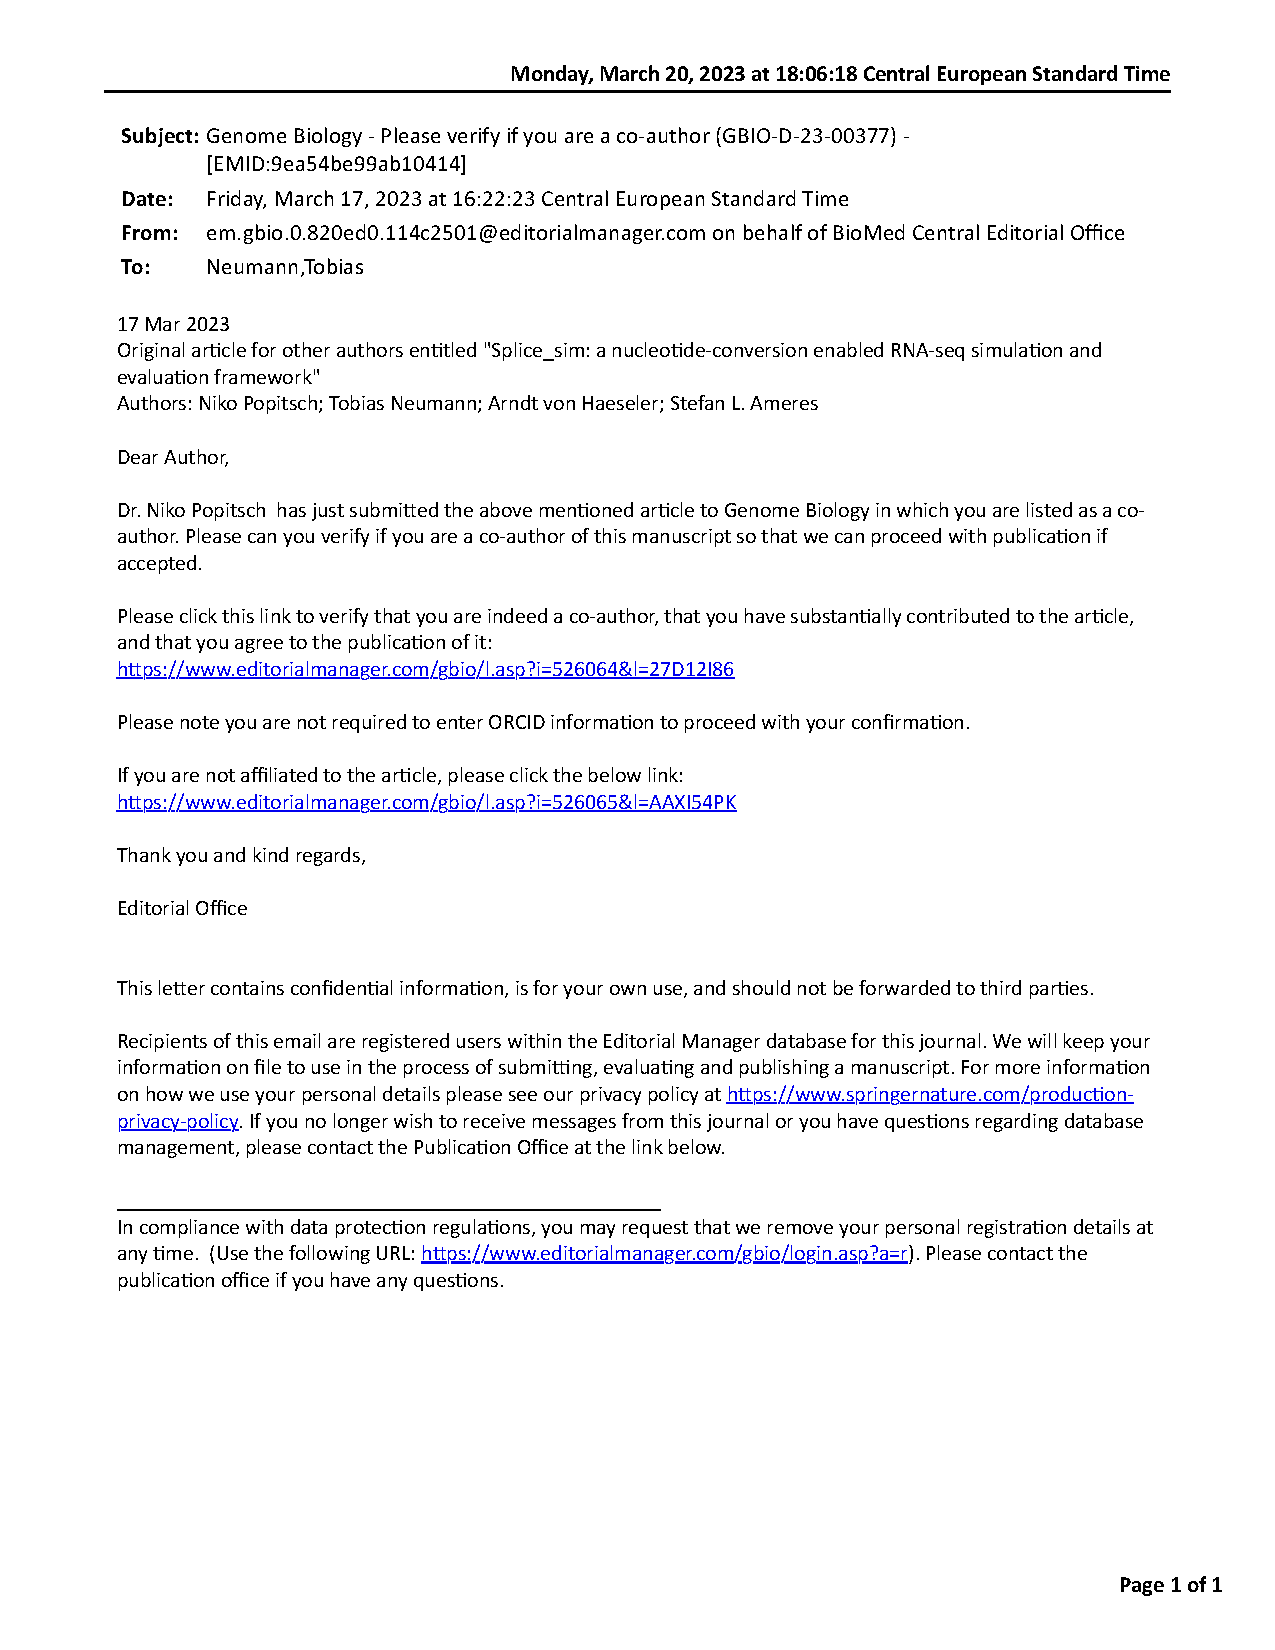
\includepdf[pages=-,frame,scale=0.7,pagecommand={}]{papers/submissionConfirmation.pdf}

\framebox[\textwidth]{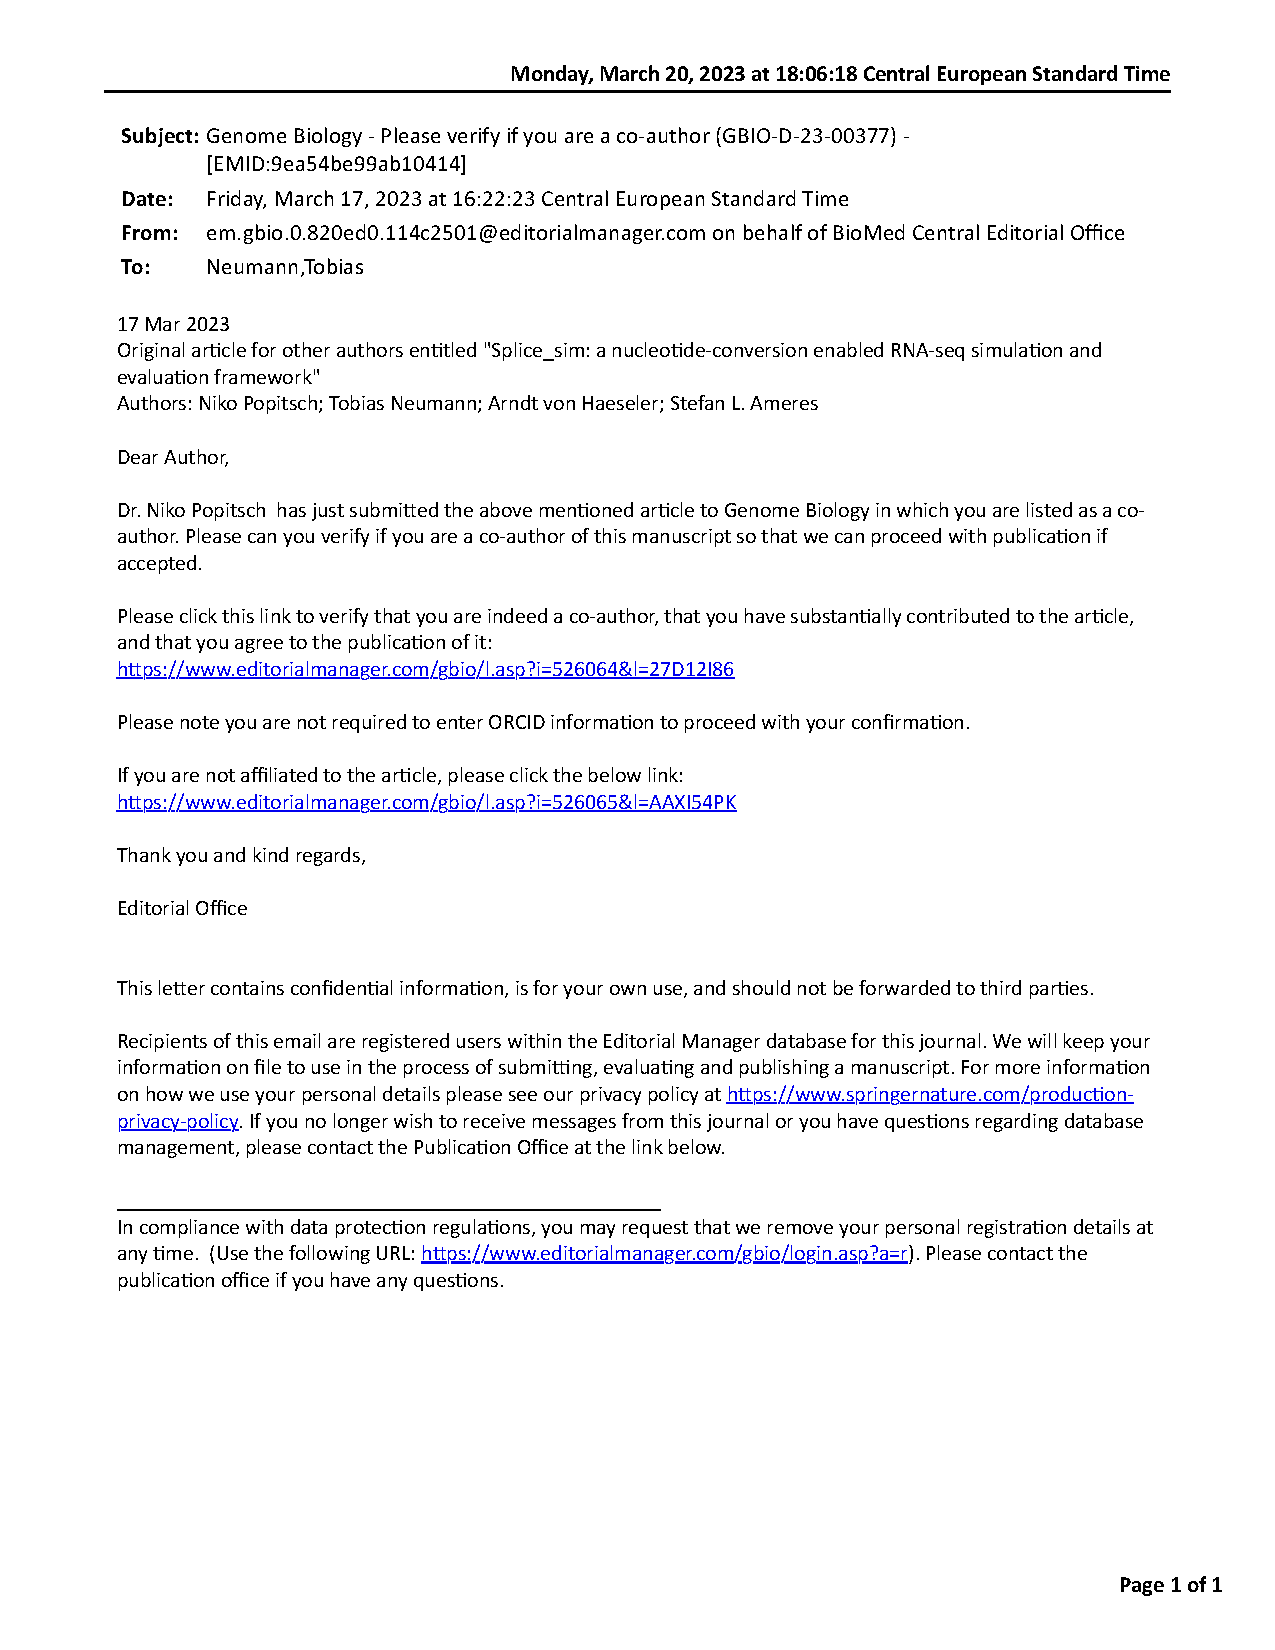
\includegraphics[page=1,scale=0.7]{papers/submissionConfirmation.pdf}}

\section{Results}

\framebox[\textwidth]{\includegraphics[page=1,scale=0.7]{papers/splice_sim_MS_final.pdf}}

\includepdf[pages=2-,frame,scale=0.7,pagecommand={}]{papers/splice_sim_MS_final.pdf}